\documentclass[a4paper,12pt]{article}
\usepackage[T2A]{fontenc}
\usepackage[utf8]{inputenc}
\usepackage[top=2cm, bottom=2cm, right=2cm, left=2cm]{geometry}
\usepackage[russian]{babel}
\usepackage{pscyr}
\usepackage{indentfirst}
\usepackage{graphicx}
\usepackage{epstopdf}
\usepackage{amstext}
\usepackage{amssymb}
\usepackage{amsmath}
\usepackage{cmap}
\usepackage{enumitem}
\usepackage{multirow}
\pdfminorversion=6
%\input{environment}
%\linespread{1.3}
\tolerance=1000 
\hfuzz=0pt
\parindent=1.27cm
\usepackage{subcaption}
\captionsetup[table]{name = Таблица, labelsep = endash, justification=raggedright, singlelinecheck=false}
\captionsetup[figure]{name = Рисунок, labelsep = endash}
\usepackage{array}
\usepackage{subcaption}
\usepackage{pgfplots}
\usetikzlibrary{pgfplots.polar}
\pgfplotsset{compat=1.13}
\pgfplotsset{grid = major, grid style = {dashed}}
\usepackage{tabu}
\usepackage{threeparttable}
\usepackage{pgfplotstable}
\renewcommand{\arraystretch}{1.5}
% recommended:
\usepackage{booktabs}
\usepackage{colortbl}
\pgfplotstableset{
	columns/w/.style = {column name = {\boldmath$\omega$}, column type = |c},
	columns/lgW/.style = {column name = {\boldmath$\lg{\omega}$}, column type = |c},
	columns/A/.style = {column name = {\boldmath$A(\omega)$}, column type = |c},
	columns/L/.style = {column name = {\boldmath$20\lg{A(\omega)}$}, column type = |c},
	columns/psi/.style = {column name = {\boldmath$\psi$}, column type = |c|},
	every head row/.style = {before row = \hline},
	after row = {[1mm] \hline},
}

%\sloppy
\RequirePackage{caption}
\DeclareCaptionLabelSeparator{defffis}{ -- }
\captionsetup{justification=centering,labelsep=defffis}
\renewcommand{\figurename}{Рисунок}
\graphicspath{{images/}{models/}}

\begin{document}
	\newcommand\tline[2]{$\underset{\text{#1}}{\text{\underline{\hspace{#2}}}}$}
	\begin{titlepage}
		\centering
		{\fontsize{12pt}{5cm}\selectfont \bfseries Министерство образования и науки Российской Федерации} \\ \vspace{0.5cm}
		{\fontsize{7pt}{5cm}\selectfont ФЕДЕРАЛЬНОЕ ГОСУДАРСТВЕННОЕ АВТОНОМНОЕ ОБРАЗОВАТЕЛЬНОЕ УЧРЕЖДЕНИЕ ВЫСШЕГО ПРОФЕССИОНАЛЬНОГО ОБРАЗОВАНИЯ} \\ 
		\vspace{1cm}
		{\fontsize{12pt}{5cm}\selectfont \bfseries САНКТ-ПЕТЕРБУРГСКИЙ УНИВЕРСИТЕТ ИНФОРМАЦИОННЫХ ТЕХНОЛОГИЙ, МЕХАНИКИ И ОПТИКИ} \\ \vspace{1.5cm}

		{\fontsize{14pt}{5cm}\selectfont Кафедра \hspace{1cm} \underline{Систем Управления и Информатики}  \hspace{1cm} Группа \underline{Р3340}} \\ 
		\vspace{2cm}

		{\fontsize{20pt}{5cm}\selectfont \bfseries Лабораторная работа №9} \\
		{\fontsize{20pt}{5cm}\selectfont \bfseries “Экспериментальное построение частотных характеристик типовых динамических звеньев”} \\
		{\fontsize{14pt}{5cm}\selectfont Вариант - 5} \\
		\vspace{1.5cm}

		\flushleft

		{Выполнил \hspace{2cm} \tline{(фамилия, и.о.)}{9cm} (подпись)} \\
		\vspace{2cm}

		{Проверил \hspace{2cm} \tline{(фамилия, и.о.)}{9cm} (подпись)} \\
		\vspace{5cm}

		"\underline{\hspace{0.7cm}}"\hspace{0.2cm}\underline{\hspace{2cm}}\hspace{0.2cm}20\underline{\hspace{0.7cm}}г. \hspace{2cm} Санкт-Петербург, \hspace{2cm} 20\underline{\hspace{0.7cm}}г. \\ \vspace{1cm}

		Работа выполнена с оценкой \hspace{1cm} \underline{\hspace{8cm}} \\ 
		\vspace{1cm}
		Дата защиты "\underline{\hspace{0.7cm}}"\hspace{0.2cm}\underline{\hspace{2cm}}\hspace{0.2cm}20\underline{\hspace{0.7cm}}г.

	\end{titlepage}
	\paragraph{Цель работы.} 	Изучение частотных характеристик типовых динамических звеньев и способов их построения. 
	\paragraph {Исходные данные:} Типы звеньев представлены в таблице \ref{t_1}. Исследования производятся при следующих коэффициентах:~$k=15$, $T=0.2$ и $\xi=0.2$.  И при гармоническом входном воздействии с единичной амплитудой и переменной частотой.
	\begin{table}[h]
		\centering
		\caption{Исходные данные}
		\renewcommand{\arraystretch}{2} 
		\renewcommand{\tabcolsep}{1.6cm}
		\begin{threeparttable}
		
		
			\begin{tabular}{|c|c|}
				
				\hline
				Тип звена & Передаточная функция \\ \hline
				Апериодическое 1го порядка & $\displaystyle W(s)=\frac{k}{Ts+1}$ \\ \hline
				Интегрирующее с замедлением & $\displaystyle W(s)=\frac{k}{s\cdot (1+Ts)}$ \\ \hline
				Изодромное & $\displaystyle W(s)=\frac{k\cdot (1+Ts)}{s}$ \\ \hline
			
		\end{tabular}
		\end{threeparttable}
		\label{t_1}
	\end{table}
	
	
	\newpage
	\begin{center}
		\section{Временная диаграмма}
	\end{center}
	\par
	Получение данных моделирования по полученной временной диаграмме, представленной на рисунке \ref{prim}, на примере апериодического звена 1го порядка при входном сигнале $g(t)=1sin(wt)$ и $w=2,k=15, T=0.2$
	\begin{figure}[h!]
		\renewcommand{\figurename}{Рисунок}
		\centering
		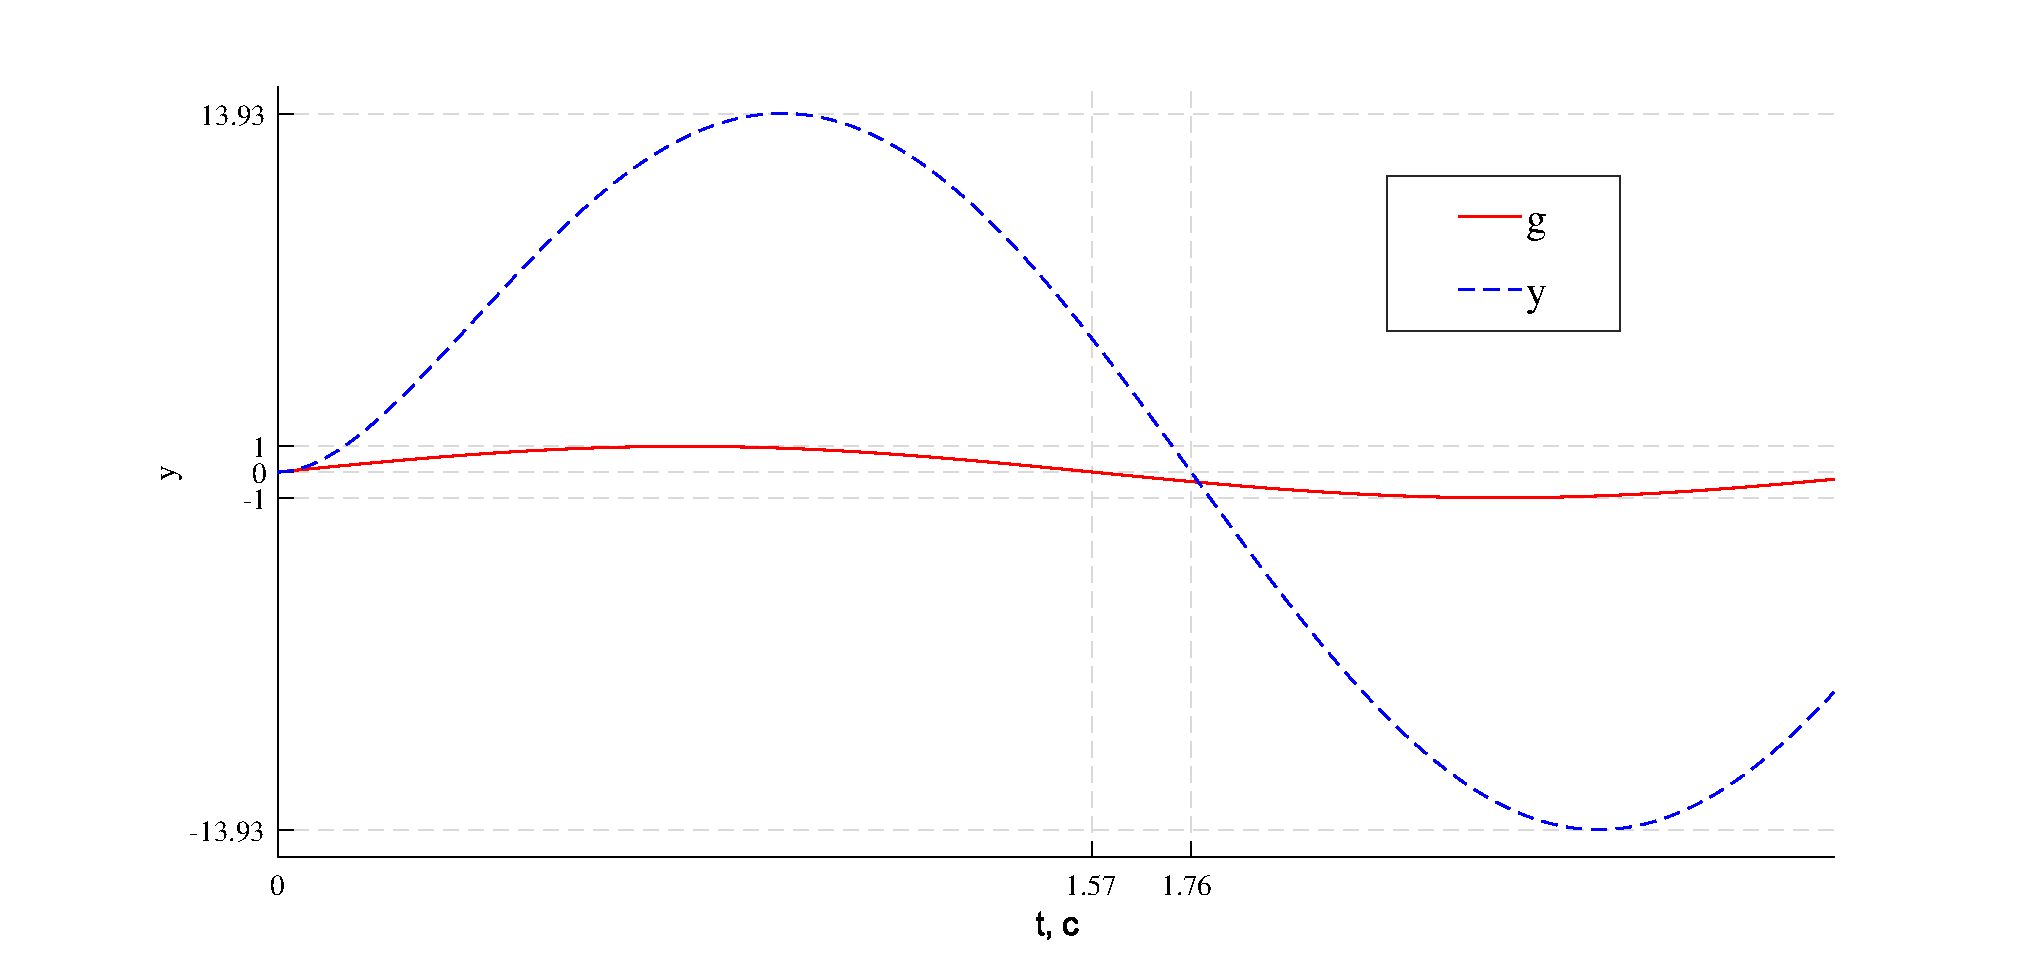
\includegraphics[width=6in]{prim.eps}
		\caption{Временная диаграмма}
		\label{prim}
	\end{figure}\\

	По рисунку видно, что амплитуда выходного сигнала $y$ равна 13.93, а амплитуда входного сигнала равна 1 $\Rightarrow A(w)=\frac{13.93}{1}=13.93$ Также видно, что входной сигнал пересекает ось времени при $t_g=1.57$, а выходной - при $t_y=1.76$, значит, $g$ опережает $y$ по фазе на угол $\phi=w\cdot \Delta t$, где $\Delta t=t_y-t_g$. Получается, фаза выходного сигнала отстает от входного $\Rightarrow \psi=-\phi$. По расчетам получается: $\Delta t = 1.76-1.57=0.19 \Rightarrow \phi=2\cdot0.19=0.38 \Rightarrow \psi=-0.38$     
	
	




	\newpage
	\begin{center}
	\section{Исследование апериодического звена 1го порядка}
	\end{center}
	\paragraph{} Данные моделирования представлены в таблице \ref{t_2}
	
		\begin{table}[h!]
			\centering
			\begin{threeparttable}
				\caption{Данные моделирования} \label{t_2}
				\pgfplotstableset{
					columns={w,lgw,A,L,psi},
					columns/w/.style = {column name = {$\omega$}, column type = |c|},
					columns/lgW/.style = {column name = {$\lg{\omega}$}, column type = |c},
					columns/A/.style = {column name = {$A(\omega)$}, column type = |c},
					columns/L/.style = {column name = {$L(w)=20\lg{A(\omega)}$}, column type = |c},
					columns/psi/.style = {column name = {$\psi(w)$}, column type = |c|},
					every head row/.style = {before row = \hline},
					after row = {[1mm] \hline},
				}
				\pgfplotstabletypeset[ % local config, applies only for this table
			1000 sep={\,},
			columns/info/.style={
				fixed,fixed zerofill,precision=1,showpos,
				column type=r,
			}
			]
			{data/NewAp1.dat}
			\end{threeparttable}
		\end{table}
	\newpage
	\paragraph{} Частотные характеристики представлены на рисунке \ref{s_1}
	\begin{figure}[h!]
		
			\renewcommand{\figurename}{Рисунок}
		\begin{subfigure}{0.5\textwidth}
			\centering
			\begin{tikzpicture}
			\begin{semilogxaxis} [
			width = 0.9\textwidth,
			xlabel = {$\omega$, 1/c},
			ylabel = {$A(w)$},
			]
			\addplot table [x={w}, y={A}] {data/NewAp1.dat};
			\end{semilogxaxis}
			\end{tikzpicture}
			\caption{АЧХ}
		\end{subfigure}
		\begin{subfigure}{0.5\textwidth}
			\centering
			\begin{tikzpicture}
			\begin{semilogxaxis} [
			width = 0.9\textwidth,
			xlabel = {$\omega$, 1/c},
			ylabel = {$\psi$, градусы},
			]
			\addplot table [x={w}, y={ugol}] {data/NewAp1.dat};
			\end{semilogxaxis}
			\end{tikzpicture}
			\caption{ФЧХ}
		\end{subfigure}
		
		\vspace{1 cm}
		
		\begin{subfigure}{0.5\textwidth}
			\centering
			\begin{tikzpicture}
			\begin{polaraxis} [
			width = 0.9\textwidth,
			xlabel = {$A(\omega)$},
			ylabel = {$\psi$, градусы},
			]
			\addplot table [x={ugol}, y={A}] {data/NewAp1.dat};
			\end{polaraxis}
			\end{tikzpicture}
			\caption{АФЧХ}
		\end{subfigure}
		\begin{subfigure}{0.5\textwidth}
			\centering
			\begin{tikzpicture}
			\begin{polaraxis} [
			width = 0.9\textwidth,
			xlabel = {$L(w)$, дБ},
			ylabel = {$\psi$, градусы},
			]
			\addplot table [x={ugol}, y={L}] {data/NewAp1.dat};
			\end{polaraxis}
			\end{tikzpicture}
			\caption{ЛАФЧХ}
		\end{subfigure}
	
		\caption{Частотные характеристики апериодического звена}
		\label{s_1}
	\end{figure}
	
	\newpage
	\begin{center}
	\section{Исследование интегрирующего с замедлением звена}
	\end{center}
	\paragraph{} Данные моделирования представлены в таблице \ref{t_3}
	\begin{table}[h!]
		\centering
		\begin{threeparttable}
		\caption{Данные моделирования} \label{t_3}
		\pgfplotstableset{
			columns={w,lgw,A,L,psi},
			columns/w/.style = {column name = {$\omega$}, column type = |c|},
			columns/lgW/.style = {column name = {$\lg{\omega}$}, column type = |c},
			columns/A/.style = {column name = {$A(\omega)$}, column type = |c},
			columns/L/.style = {column name = {$L(w)=20\lg{A(\omega)}$}, column type = |c},
			columns/psi/.style = {column name = {$\psi(w)$}, column type = |c|},
			every head row/.style = {before row = \hline},
			after row = {[1mm] \hline},
		}
		\pgfplotstabletypeset[ % local config, applies only for this table
		1000 sep={\,},
		columns/info/.style={
			fixed,fixed zerofill,precision=1,showpos,
			column type=r,
		}
		]
		{data/NewIntegrszamed.dat}
		\end{threeparttable}
	\end{table}
	\newpage
	\paragraph{} Частотные характеристики представлены на рисунке \ref{s_2}
	\begin{figure}[h!]
		
		\renewcommand{\figurename}{Рисунок}
		\begin{subfigure}{0.5\textwidth}
			\centering
			\begin{tikzpicture}
			\begin{semilogxaxis} [
			width = 0.9\textwidth,
			xlabel = {$\omega$, 1/c},
			ylabel = {$A(w)$},
			]
			\addplot table [x={w}, y={A}] {data/NewIntegrszamed.dat};
			\end{semilogxaxis}
			\end{tikzpicture}
			\caption{АЧХ}
		\end{subfigure}
		\begin{subfigure}{0.5\textwidth}
			\centering
			\begin{tikzpicture}
			\begin{semilogxaxis} [
			width = 0.9\textwidth,
			xlabel = {$\omega$, 1/c},
			ylabel = {$\psi$, градусы},
			]
			\addplot table [x={w}, y={ugol}] {data/NewIntegrszamed.dat};
			\end{semilogxaxis}
			\end{tikzpicture}
			\caption{ФЧХ}
		\end{subfigure}
		
		\vspace{1 cm}
		
		\begin{subfigure}{0.5\textwidth}
			\centering
			\begin{tikzpicture}
			\begin{polaraxis} [
			width = 0.9\textwidth,
			xlabel = {$A(\omega)$},
			ylabel = {$\psi$, градусы},
			]
			\addplot table [x={ugol}, y={A}] {data/NewIntegrszamed.dat};
			\end{polaraxis}
			\end{tikzpicture}
			\caption{АФЧХ}
		\end{subfigure}
		\begin{subfigure}{0.5\textwidth}
			\centering
			\begin{tikzpicture}
			\begin{polaraxis} [
			width = 0.9\textwidth,
			xlabel = {$L(w)$, дБ},
			ylabel = {$\psi$, градусы},
			]
			\addplot table [x={ugol}, y={L}] {data/NewIntegrszamed.dat};
			\end{polaraxis}
			\end{tikzpicture}
			\caption{ЛАФЧХ}
		\end{subfigure}
		
		\caption{Частотные характеристики интегрирующего с замедлением звена}
		\label{s_2}
	\end{figure}
	
	
	\newpage
	\begin{center}
	\section{Исследование изодромного звена}
	\end{center}
	\paragraph{} Данные моделирования представлены в таблице \ref{t_4}
	\begin{table}[h!]
		\centering
		\begin{threeparttable}
		\caption{Данные моделирования} \label{t_4}
		\pgfplotstableset{
		columns={w,lgw,A,L,psi},
		columns/w/.style = {column name = {$\omega$}, column type = |c|},
		columns/lgW/.style = {column name = {$\lg{\omega}$}, column type = |c},
		columns/A/.style = {column name = {$A(\omega)$}, column type = |c},
		columns/L/.style = {column name = {$L(w)=20\lg{A(\omega)}$}, column type = |c},
		columns/psi/.style = {column name = {$\psi(w)$}, column type = |c|},
		every head row/.style = {before row = \hline},
		after row = {[1mm] \hline},
	}
		\pgfplotstabletypeset[ % local config, applies only for this table
		1000 sep={\,},
		columns/info/.style={
			fixed,fixed zerofill,precision=1,showpos,
			column type=r,
		}
		]
		{data/NewIzodrom.dat}
		\end{threeparttable}
	\end{table}
	\newpage
	\paragraph{} Частотные характеристики представлены на рисунке \ref{s_3}
	\begin{figure}[h!]
	
		\renewcommand{\figurename}{Рисунок}
		\begin{subfigure}{0.5\textwidth}
			\centering
			\begin{tikzpicture}
			\begin{semilogxaxis} [
			width = 0.9\textwidth,
			xlabel = {$\omega$, 1/c},
			ylabel = {$A(w)$},
			]
			\addplot table [x={w}, y={A}] {data/NewIzodrom.dat};
			\end{semilogxaxis}
			\end{tikzpicture}
			\caption{АЧХ}
		\end{subfigure}
		\begin{subfigure}{0.5\textwidth}
			\centering
			\begin{tikzpicture}
			\begin{semilogxaxis} [
			width = 0.9\textwidth,
			xlabel = {$\omega$, 1/c},
			ylabel = {$\psi$, градусы},
			]
			\addplot table [x={w}, y={ugol}] {data/NewIzodrom.dat};
			\end{semilogxaxis}
			\end{tikzpicture}
			\caption{ФЧХ}
		\end{subfigure}
		
		\vspace{1 cm}
		
		\begin{subfigure}{0.5\textwidth}
			\centering
			\begin{tikzpicture}
			\begin{polaraxis} [
			width = 0.9\textwidth,
			xlabel = {$A(\omega)$},
			ylabel = {$\psi$, градусы},
			]
			\addplot table [x={ugol}, y={A}] {data/NewIzodrom.dat};
			\end{polaraxis}
			\end{tikzpicture}
			\caption{АФЧХ}
		\end{subfigure}
		\begin{subfigure}{0.5\textwidth}
			\centering
			\begin{tikzpicture}
			\begin{polaraxis} [
			width = 0.9\textwidth,
			xlabel = {$L(w)$, дБ},
			ylabel = {$\psi$, градусы},
			]
			\addplot table [x={ugol}, y={L}] {data/NewIzodrom.dat};
			\end{polaraxis}
			\end{tikzpicture}
			\caption{ЛАФЧХ}
		\end{subfigure}
		
		\caption{Частотные характеристики изодромного звена}
			\label{s_3}
	\end{figure}
	
	\newpage
	\begin{center}
	\section{Асимптотические ЛАЧХ исследуемых звеньев}
	\end{center}
	\paragraph{}
	На рисунках \ref{s_4}, \ref{s_5} и \ref{s_6} представлены асимптотические и полученные моделированием ЛАЧХ для апериодического, интегрирующего с замедлением и изодромного звена соответственно.
	\begin{figure}[h!]
		
		\renewcommand{\figurename}{Рисунок}
		
			\centering
			\begin{tikzpicture}
			\begin{semilogxaxis} [
			width = 0.9\textwidth,
			ylabel = {$L(w)$, дБ},
			xlabel = {$w$, рад/c},
			]
			\addplot table [x={w}, y={L}] {data/NewAp1.dat};
			\addplot [red, thick, mark = none, style = dashed] table [x={w}, y={L}] {data/AsimptAper1.dat};
			\legend{\text{\scriptsize Моделирование}, \text{\scriptsize Теория}}
			\end{semilogxaxis}
			\end{tikzpicture}
				\caption{ЛАЧХ апериодического звена 1го порядка}
				\label{s_4}
		\end{figure}
		
		\begin{figure}[h!]
			\centering
			\begin{tikzpicture}
			\begin{semilogxaxis} [
			width = 0.9\textwidth,
			ylabel = {$L(w)$, дБ},
			xlabel = {$w$, рад/c},
			]
			\addplot table [x={w}, y={L}] {data/NewIntegrszamed.dat};
			\addplot [red, thick, mark = none, style = dashed] table [x={w}, y={L}] {data/AsimptIntegrszamed.dat};
			\legend{\text{\scriptsize Моделирование}, \text{\scriptsize Теория}}
			\end{semilogxaxis}
			\end{tikzpicture}
			\caption{ЛАЧХ интегрирующего с замедлением звена}
			\label{s_5}
	\end{figure}
		\begin{figure}[h!]
			
				\centering
				\begin{tikzpicture}
				\begin{semilogxaxis} [
				width = 0.9\textwidth,
				ylabel = {$L(w)$, дБ},
				xlabel = {$w$, рад/c},
				]
				\addplot table [x={w}, y={L}] {data/NewIzodrom.dat};
				\addplot [red, thick, mark = none, style = dashed] table [x={w}, y={L}] {data/AsimptIzodrom.dat};
				\legend{\text{\scriptsize Моделирование}, \text{\scriptsize Теория}}
				\end{semilogxaxis}
				\end{tikzpicture}
		
		\caption{ЛАЧХ изодромного звена}
		\label{s_6}
	\end{figure}


	\clearpage
	\begin{center}
	\section*{Вывод}
	\end{center}
	
	В данной работе были исследованы три динамических звена: апериодическое 1го порядка, интегрирующее с замедлением и изодромное. В результате были получены частотные характеристики, по которым можно судить о значениях амплитуды и фазы выходного сигнала звена в зависимости от параметров входного сигнала. Также были построены теоретические асимптотические ЛАЧХ, которые подтвердили данные, полученные моделированием.

\end{document}